\documentclass[Softwaredesign/Softwaredesign_main.tex]{subfiles}

\begin{document}

\section{GUI user interface desgin}
\begin{figure}[H]
    \centering
    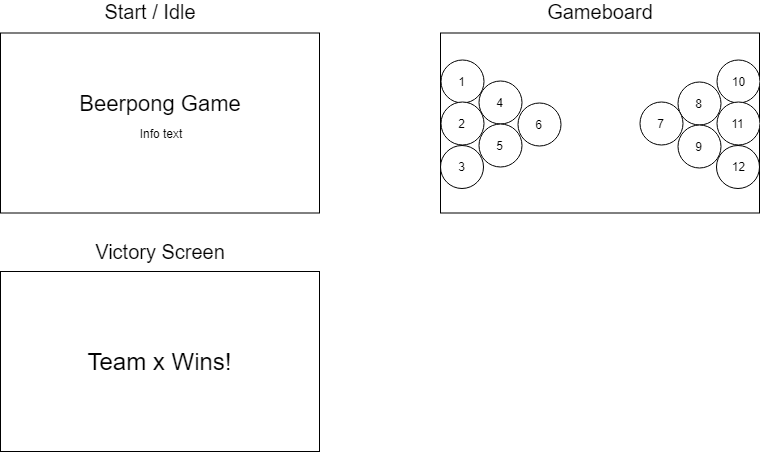
\includegraphics[scale=0.5]{Softwaredesign/GUI/Pictures/Boards.png}
    \caption{Forskellige design af "Game boards"}
    \label{gameboards}
\end{figure}

På figur \ref{gameboards} kan de forskellige "states" som displayet vil vise ses. Der er et "Start/Idle" state. Dette er den state som displayet vil vise når der intet spil er igangværende, det ville svare til en låsskærm på en telefon/PC. På skærmen vil der stå navnet på spillet "Beerpong Game"; samt en tilhørende mindre tekst: Waiting for a new game to start". 
\\Derefter ses "Gameboard" state. Det er det state som skærmen vil være i når et spil er igangværende. Det vil sige at når der startes et nyt spil går den fra "Start/Idle", over til "Gameboard". Der vil der vises det forskellige kopper: fra 1 til og med 12. Disse ringe har enten en "off" farve (rød), eller en "on" farve (grøn). Desuden er er en tekst streng; denne tekst indeholder beskeder til spilleren. Dette kan være: "Stil alle kopperne på plads for at starte stil", "Kop x ramt", "Fjern kop x": X værende et vilkærligt tal mellem 1 og 12. 
\\ 
Til sidst er der "Victory Screen". Dette er state displayet viser når et hold vinder. Det vil sige at den går fra "Gameboard" staten, hen til "Victory Screen" staten. På skærmen vises der en tekst som viser hvilket hold som har vundet spillet. Denne skærm er der så i 10 sekunder, hvor efter den skifter tilbage til "Start/Idle" state.  
\\
Et state machine diagram som viser det ovenforforklarede kan ses på figur \ref{GuiDisplayStatemachine}

\begin{figure}[H]
    \centering
    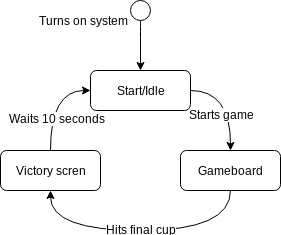
\includegraphics{Softwaredesign/GUI/Pictures/GuiDisplayStatemachine.png}
    \caption{Statemachine for display tilstand}
    \label{GuiDisplayStatemachine}
\end{figure}


\end{document}